\providecommand{\main}{../../../..}
\documentclass[\main/dresen_thesis.tex]{subfiles}

\begin{document}
  \label{sec:monolayers:preparation:solventProperties}
  \begin{figure}[tb]
    \centering
    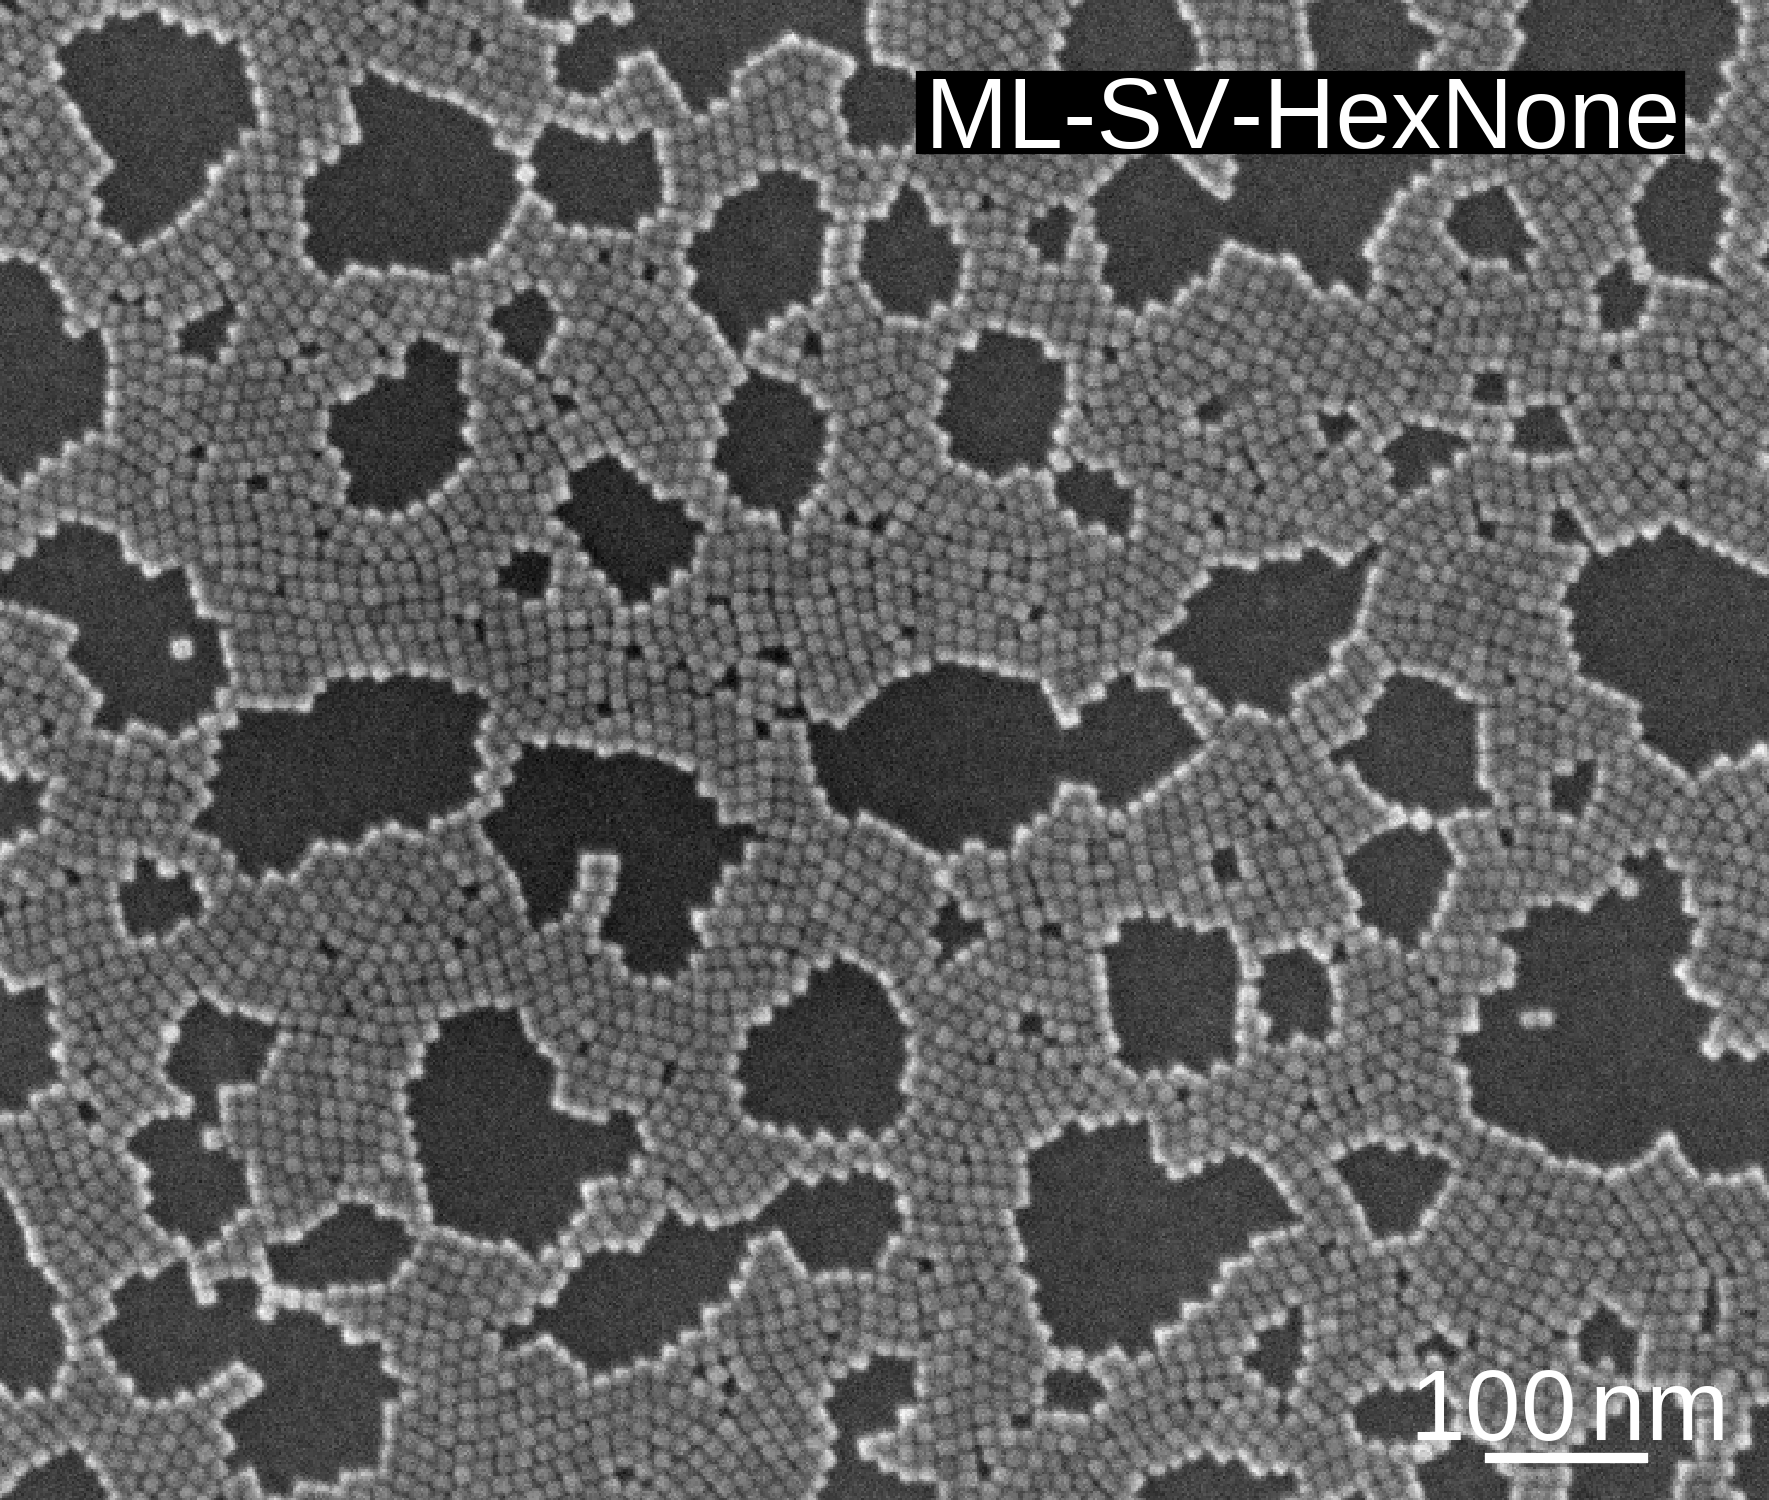
\includegraphics{monolayers_SEM_ML-SV-HexNone}
    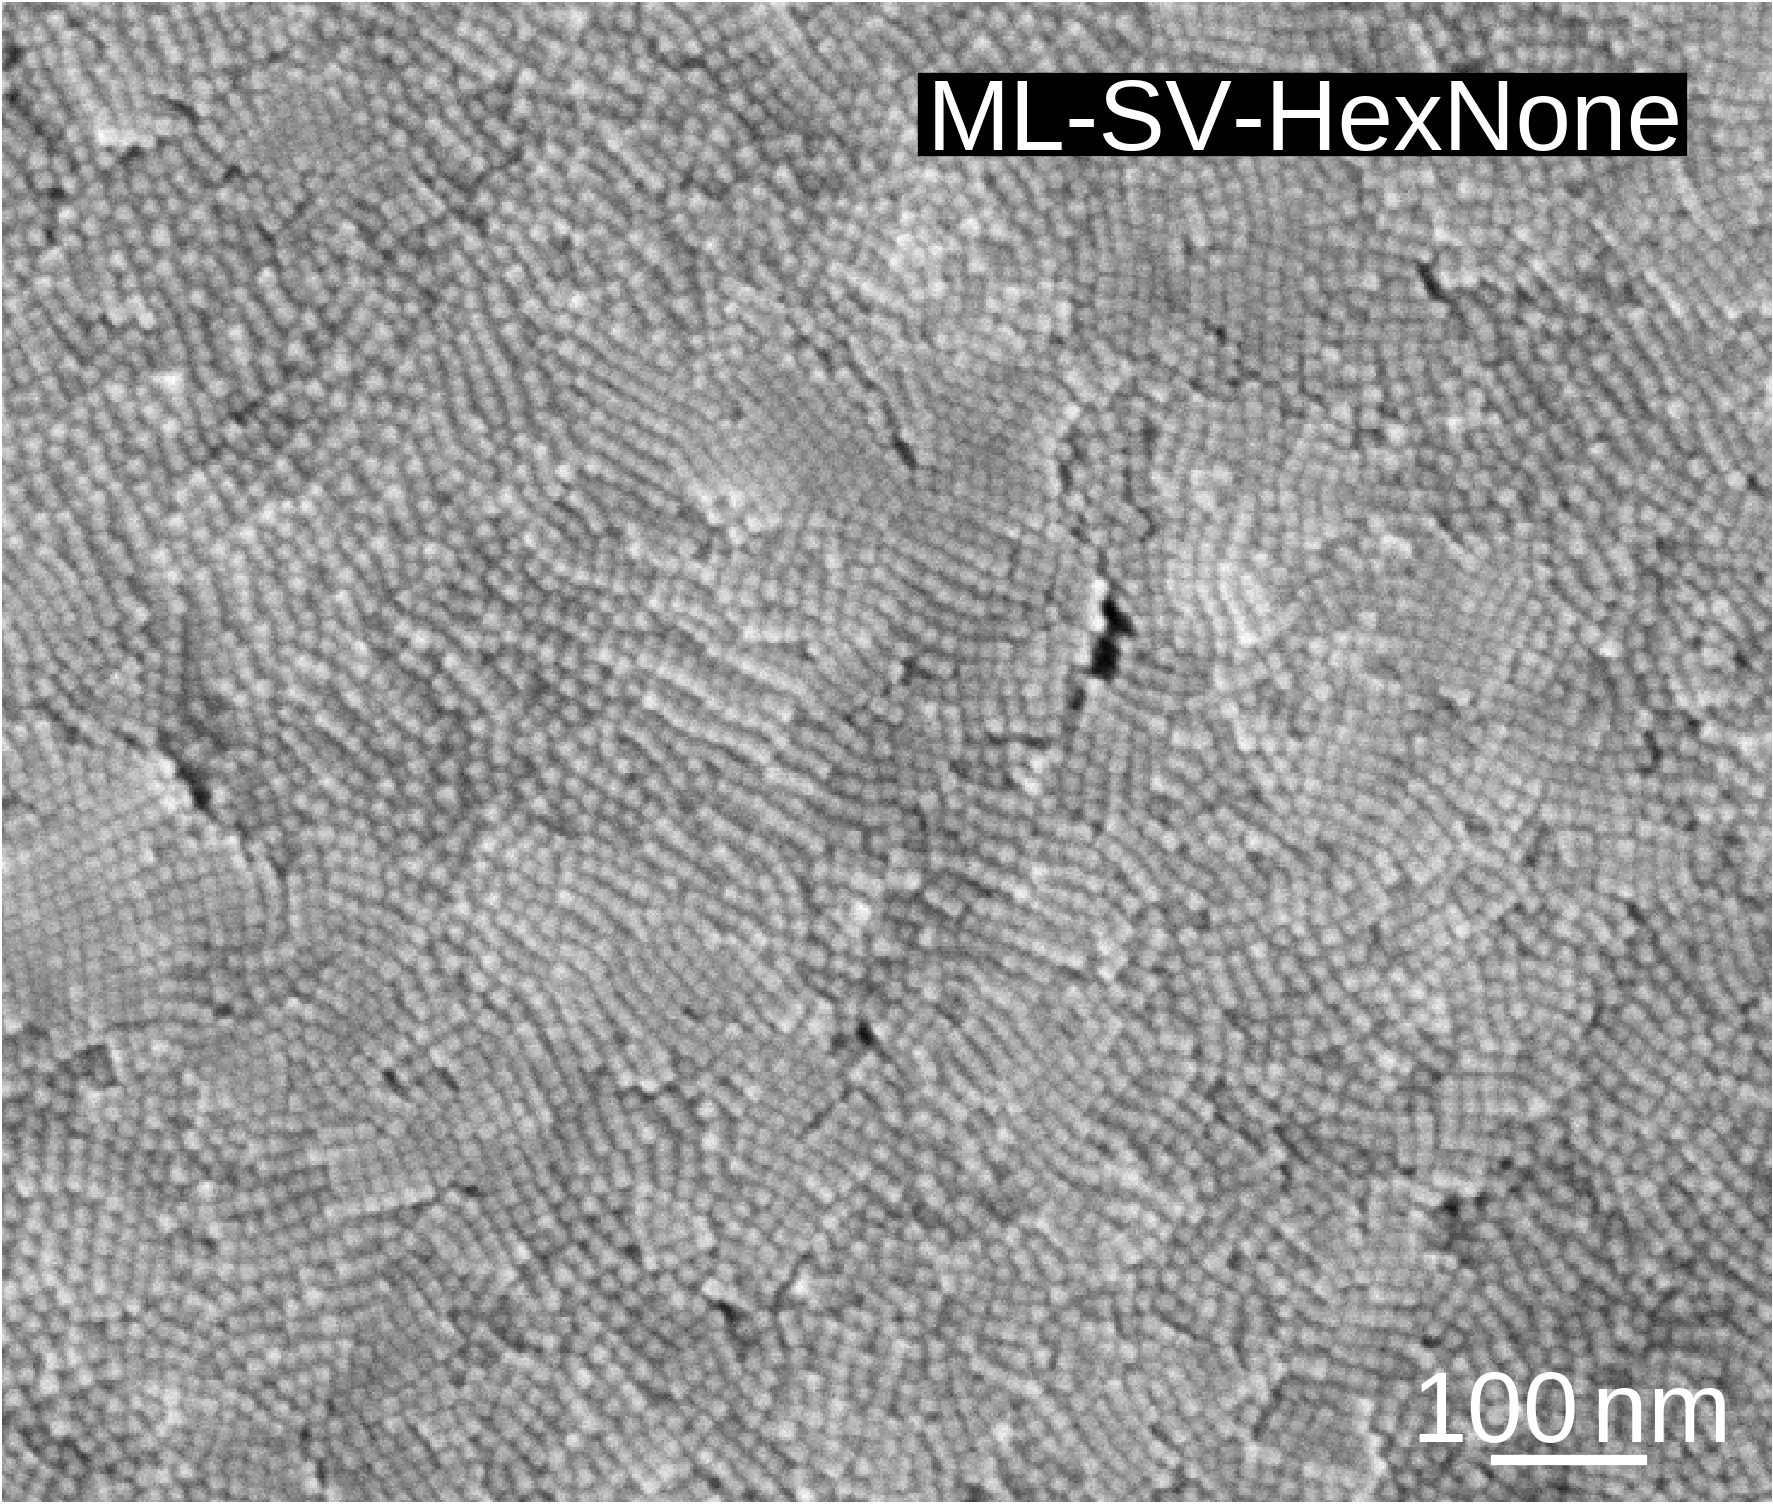
\includegraphics{monolayers_SEM_ML-SV-HexNone2}
    \caption{\label{fig:monolayers:preparation:solventVariation:semNoCoSolvent}SEM micrograph of Ol-CoFe-C nanoparticles after drop casting from $\mathit{n}$-hexane and without a co-solvent additive from two different positions at the center of the same substrate.}
  \end{figure}
  The solvent and co-solvent of the dispersion for the drop casting experiment determine the mobility of the nanoparticles and the time scales for a drop casting experiment.
  When oleic acid ligated nanocubes are drop casted as-prepared at low concentration from an organic dispersion such as \textit{n}-hexane without any additional additives or setups, no long-range order is observed and the overall sample quality is inhomogeneous as seen in \reffig{fig:monolayers:preparation:solventVariation:semNoCoSolvent}.
  On different positions of the substrate, the nanoparticles have either connected with many holes in between or they are heaped in a bulk, showing in both cases only short-range order.
  This observation suggests sub-optimal wetting conditions for the solvent and a missing mechanism in the self-assembly process for an even distribution of the particles across the substrate.
  Therefore, the effect of adding co-solvents and variation of the primary solvent on the nanoparticle self-organization is studied in detail.

  \subsubsection{Alkanes / Alkenes as Solvent / Co-Solvent}
    To study the effect of the solvent choice on the structural long-range order for drop casted nanocubes, a series of  primary/co-solvent mixtures are studied by performing drop casting experiments with the nanocubes Ol-CoFe-C.
    In the following four combinations solvent/co-solvent combinations are discussed in detail: A sample of an alkene with a relatively low boiling point, 1-tetradecene ($T_\mathrm{bp} \eq 251 \unit{^\circ C}$), together with \textit{n}-hexane (ML-SV-HexTet), and three samples of 1-octadecene ($T_\mathrm{bp} \eq 315 \unit{^\circ C}$) with varied alkanes \textit{n}-pentane (ML-SV-PenOct), \textit{n}-hexane (ML-SV-HexOct) and \textit{n}-heptane (ML-SV-HepOct).

    \begin{figure}[tb]
      \centering
      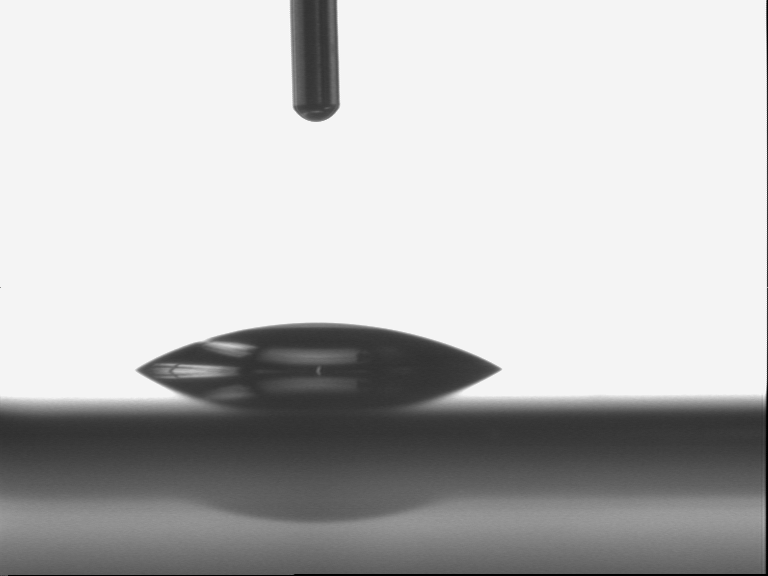
\includegraphics[width=0.31\textwidth]{monolayer_contactAngle_Water}
      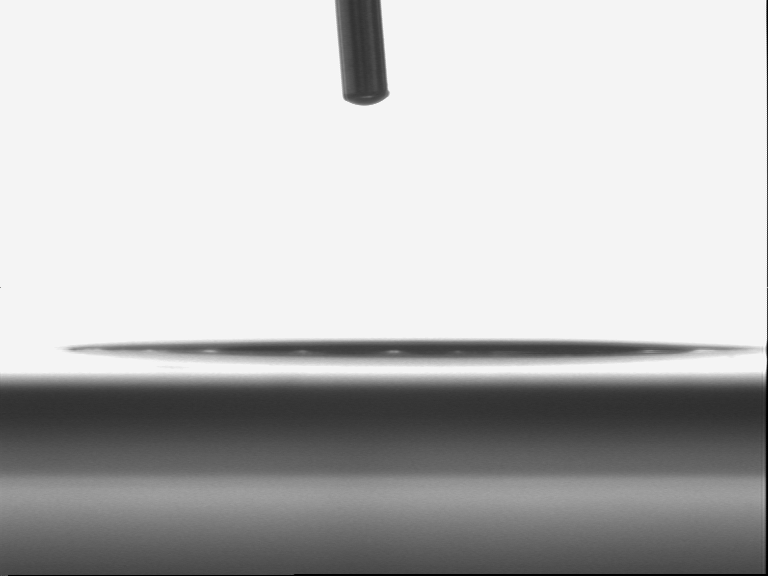
\includegraphics[width=0.31\textwidth]{monolayer_contactAngle_OlCoFeC}
      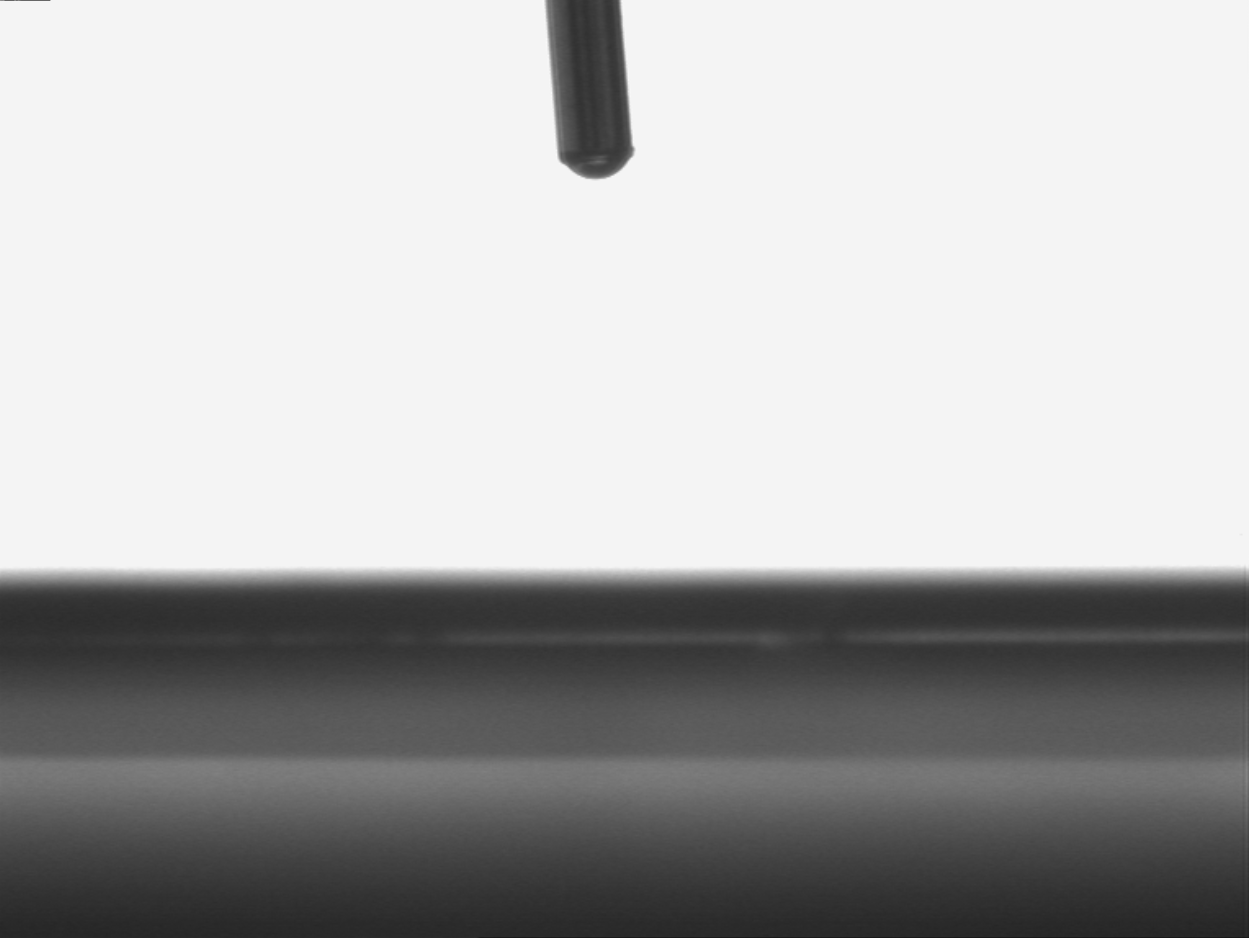
\includegraphics[width=0.31\textwidth]{monolayer_contactAngle_OlCoFeCOctadecene2Percent}
      \caption{\label{fig:monolayers:preparation:contactAngle}Side-view camera image of a droplet of water (left), a droplet of $\mathit{n}$-hexane (center) and a droplet of $\mathit{n}$-hexane with $2 \unit{\%}$ 1-octadecene (right) on a silicon substrate.}
    \end{figure}
    An effect of the co-solvent additive that is immediately visible during the drop casting procedure is the improved wetting of the dispersion on the substrate.
    Attempts to measure the contact angle between dispersion and silicon substrate are shown in \reffig{fig:monolayers:preparation:contactAngle} in comparison to a droplet of water on silicon.
    While the contact angle of $\mathit{n}$-hexane is $<10^\circ$ on silicon, the addition of a small amount of octadecene as additive makes the droplet no longer visible in a side view meaning that it evenly spreads on the surface.
    This indicates that the alkene additive greatly increases the wetting properties of the dispersion.

    \begin{figure}[tb]
      \centering
      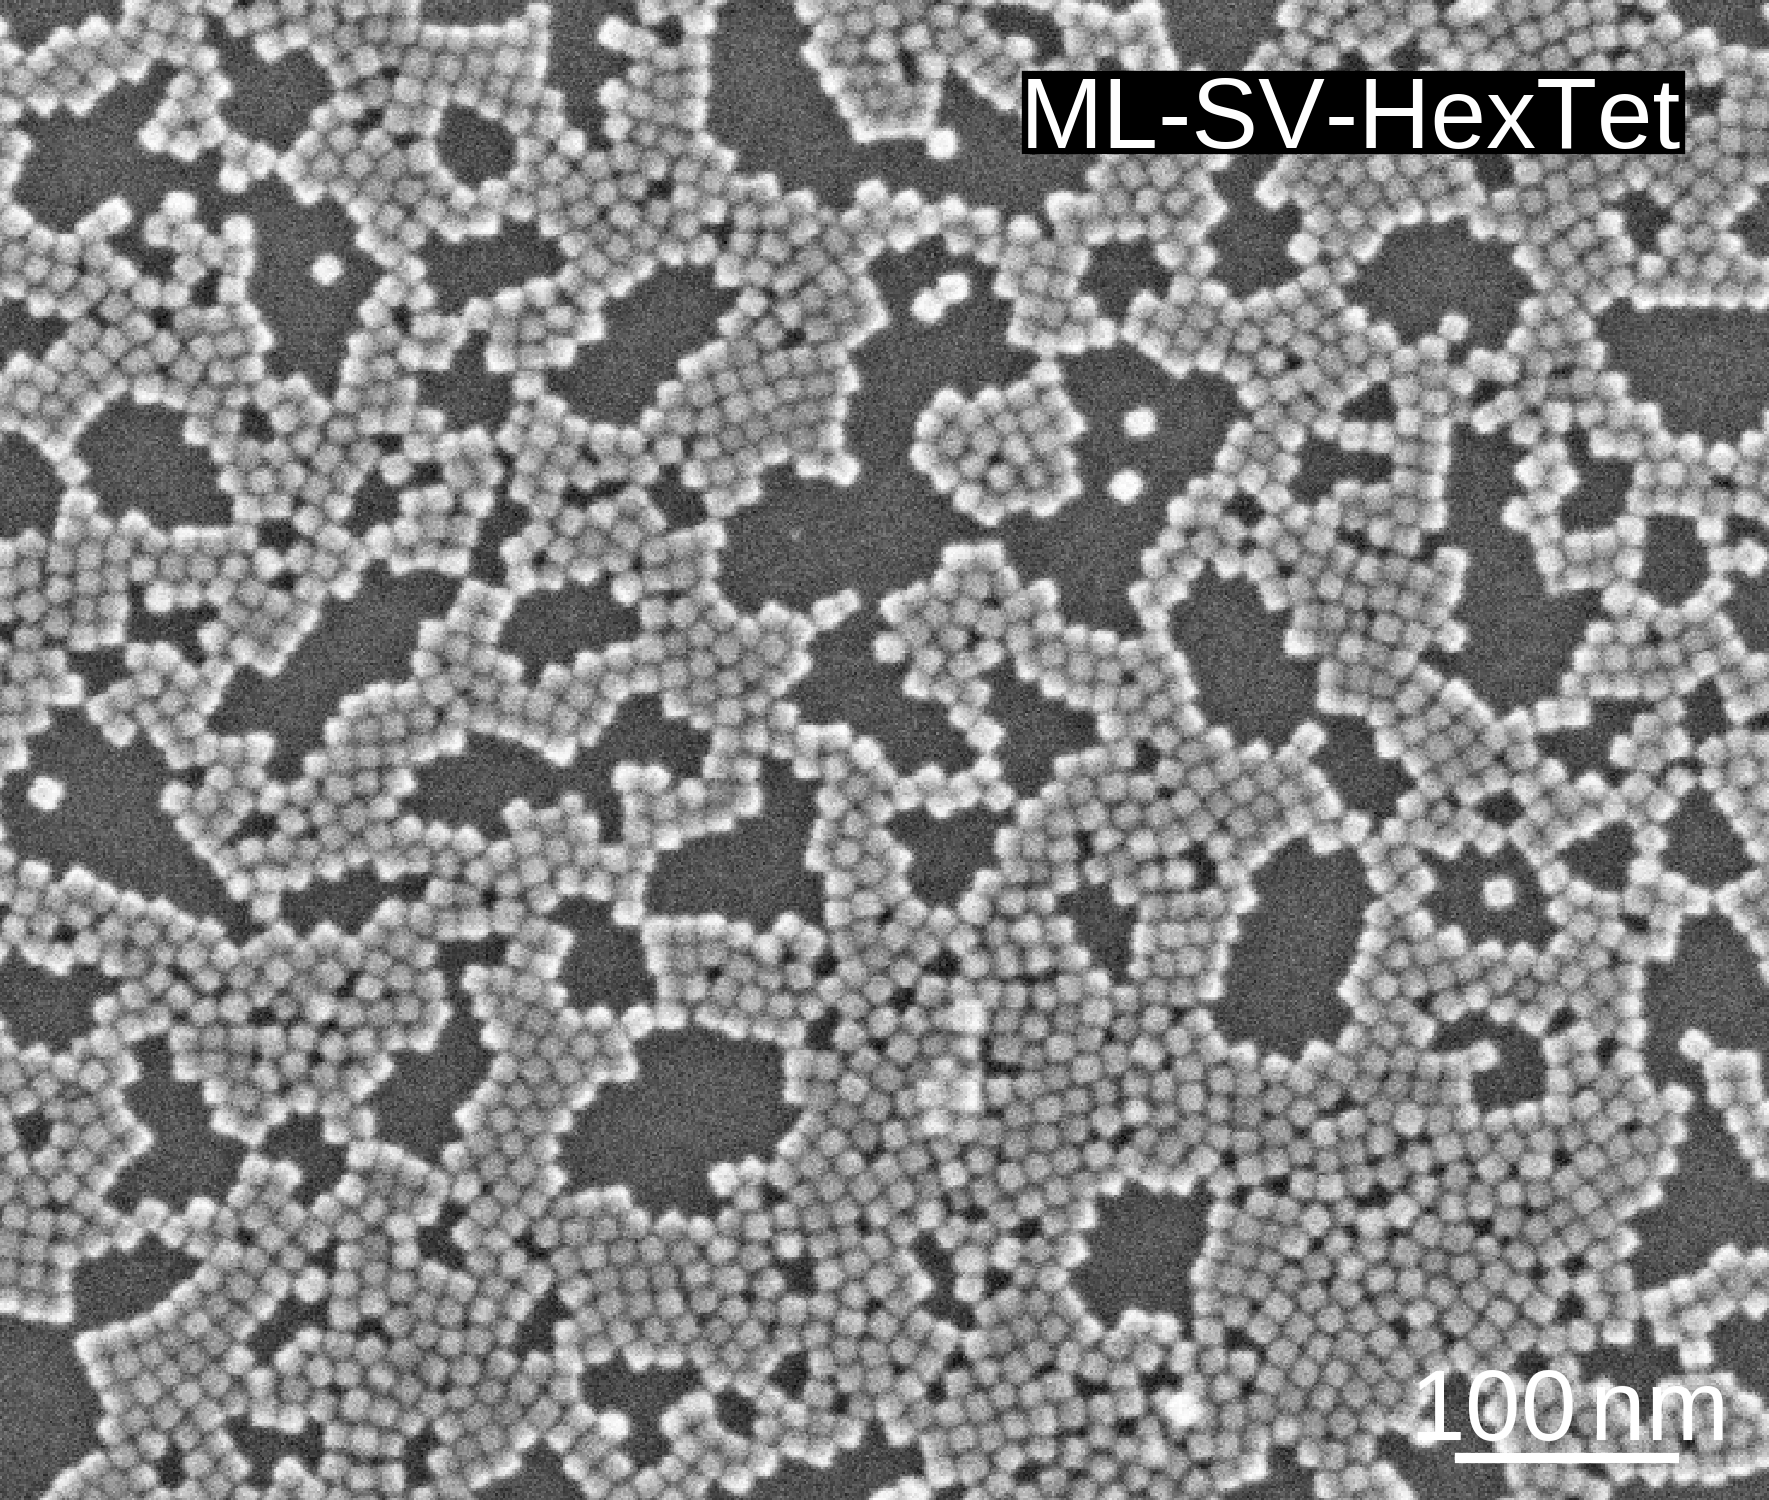
\includegraphics{monolayers_SEM_ML-SV-HexTet}
      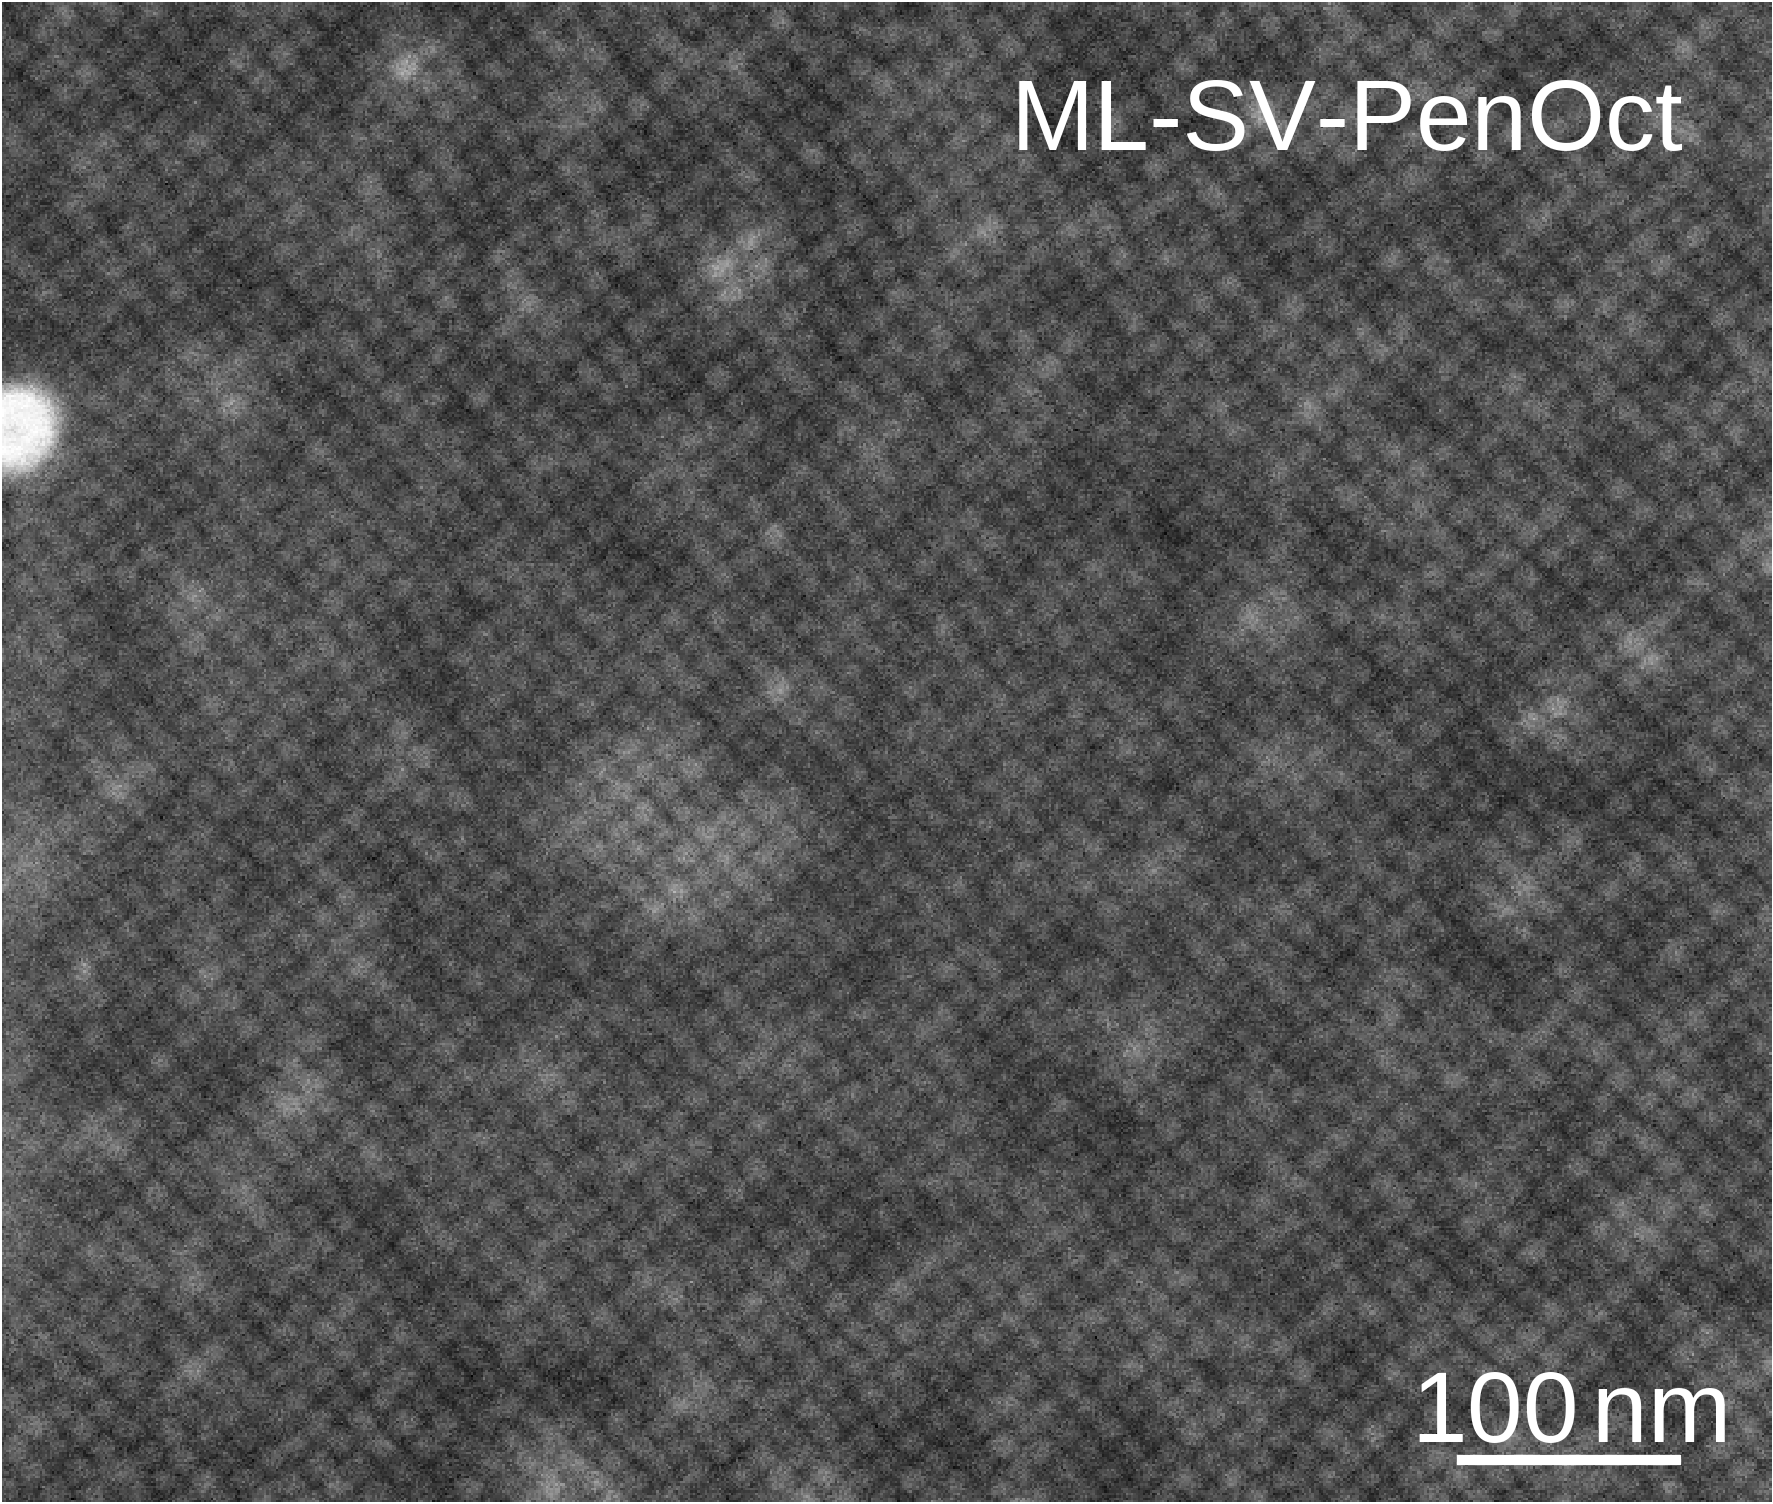
\includegraphics{monolayers_SEM_ML-SV-PenOct}
      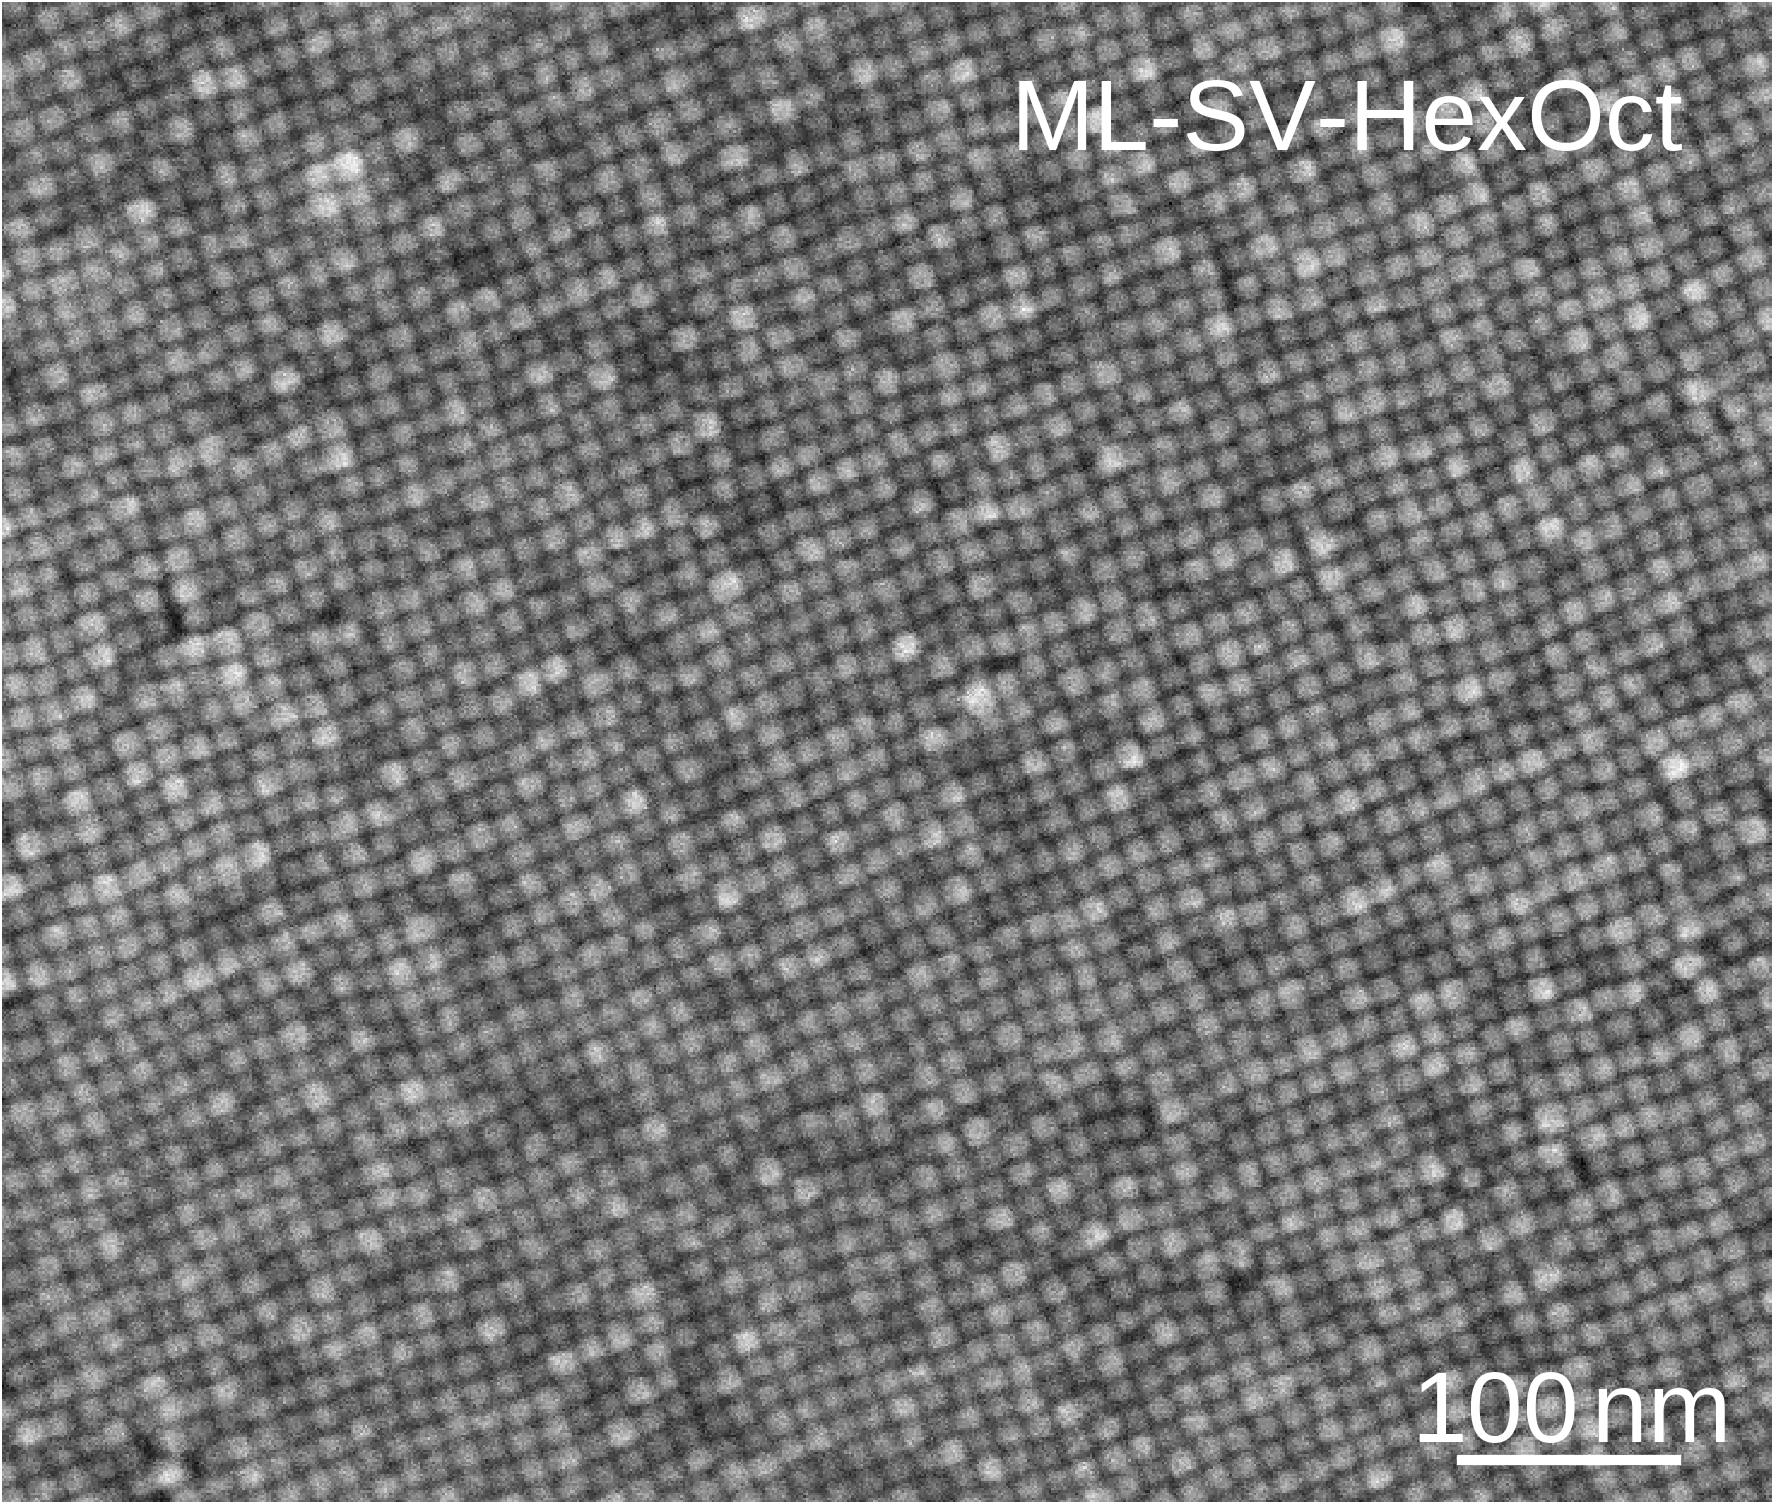
\includegraphics{monolayers_SEM_ML-SV-HexOct}
      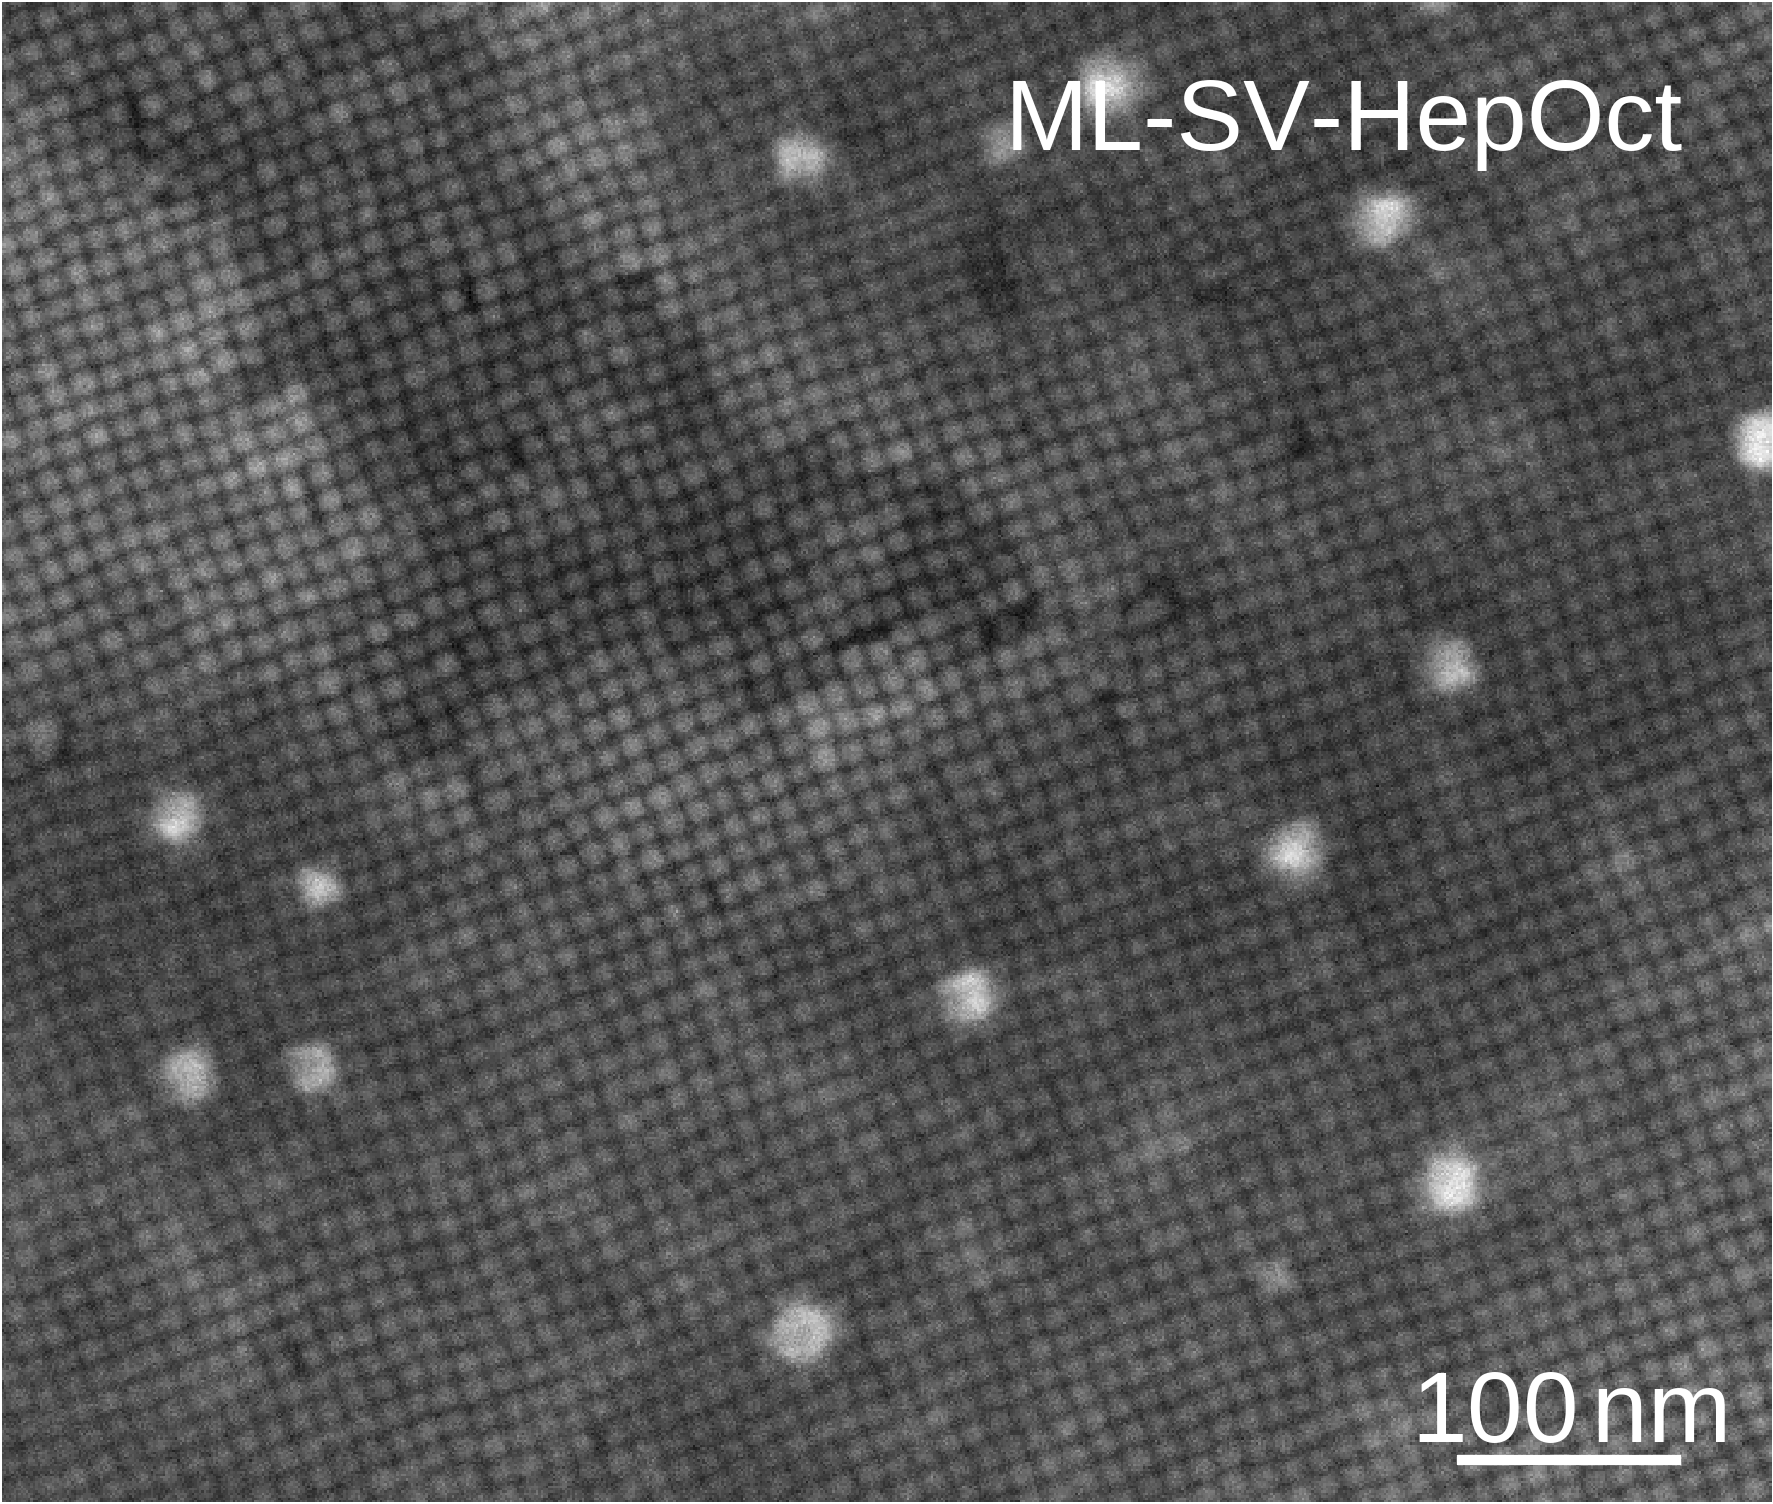
\includegraphics{monolayers_SEM_ML-SV-HepOct}
      \caption{\label{fig:monolayers:preparation:solventVariation:sem}Scanning electron microscopy of Ol-CoFe-C nanoparticles after drop casting using $\mathit{n}$-hexane/tetradecene (upper left), $\mathit{n}$-pentane/octadecene (upper right), $\mathit{n}$-hexane/octadecene (lower left) and $\mathit{n}$-heptane/octadecene (lower right) as solvents.}
    \end{figure}
    In \reffig{fig:monolayers:preparation:solventVariation:sem} SEM micrographs of the four drop casted solvent/co-solvent combinations are presented.
    It is imminently visible that an alkene with a relatively low boiling point such as 1-tetradecene leads to no order formation, whereas  combinations with 1-octadecene show for all alkanes local square order formation.

    The micrographs of ML-SV-PenOct and ML-SV-HepOct further reveals small bright spots on top of the ordered nanoparticles.
    Closer inspection of the spots by using the scanning electron microscope show that these spots can be melted with the electron beam.
    This indicates that the spots are possible organic remnants that are dissolved by the high energy of the electron beam.
    As the substrates have been baked for several hours at elevated temperatures of $140 \unit{^\circ C}$ prior the measurement and as the SEM has a ultra-high vacuum during the measurements, these dissolvable organic compounds must have a low vapor pressure to resist removal.
    Considering the involved organic materials, the bright spots are most likely remnants of either octadecene or oleic acid.


    \begin{figure}[tb]
      \centering
      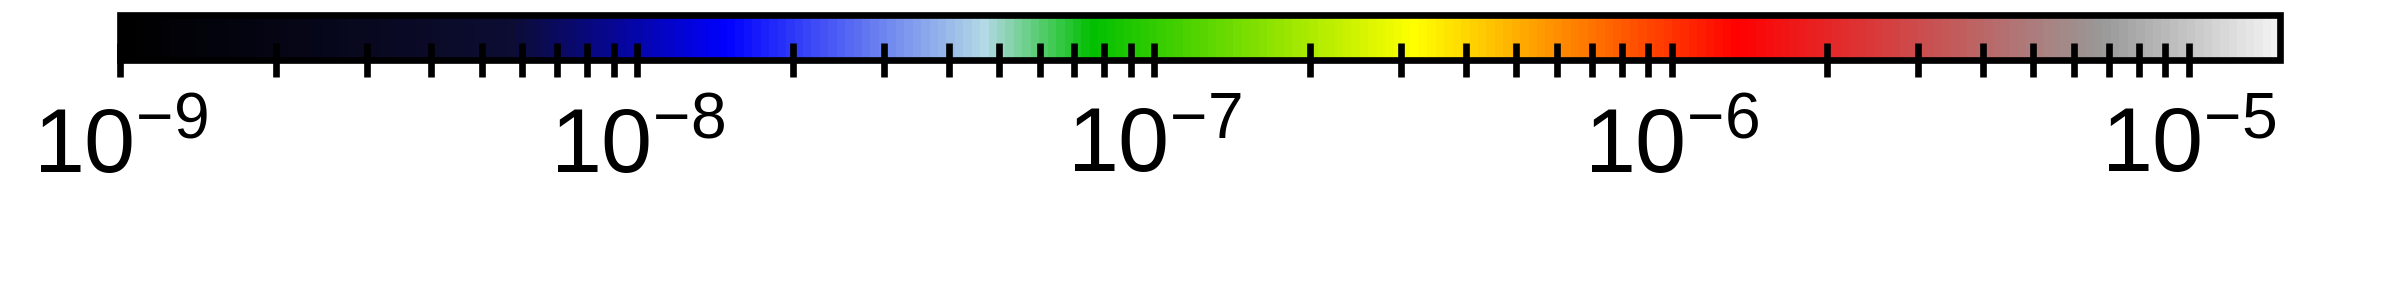
\includegraphics{monolayers_GISAXS_SVcbar}
      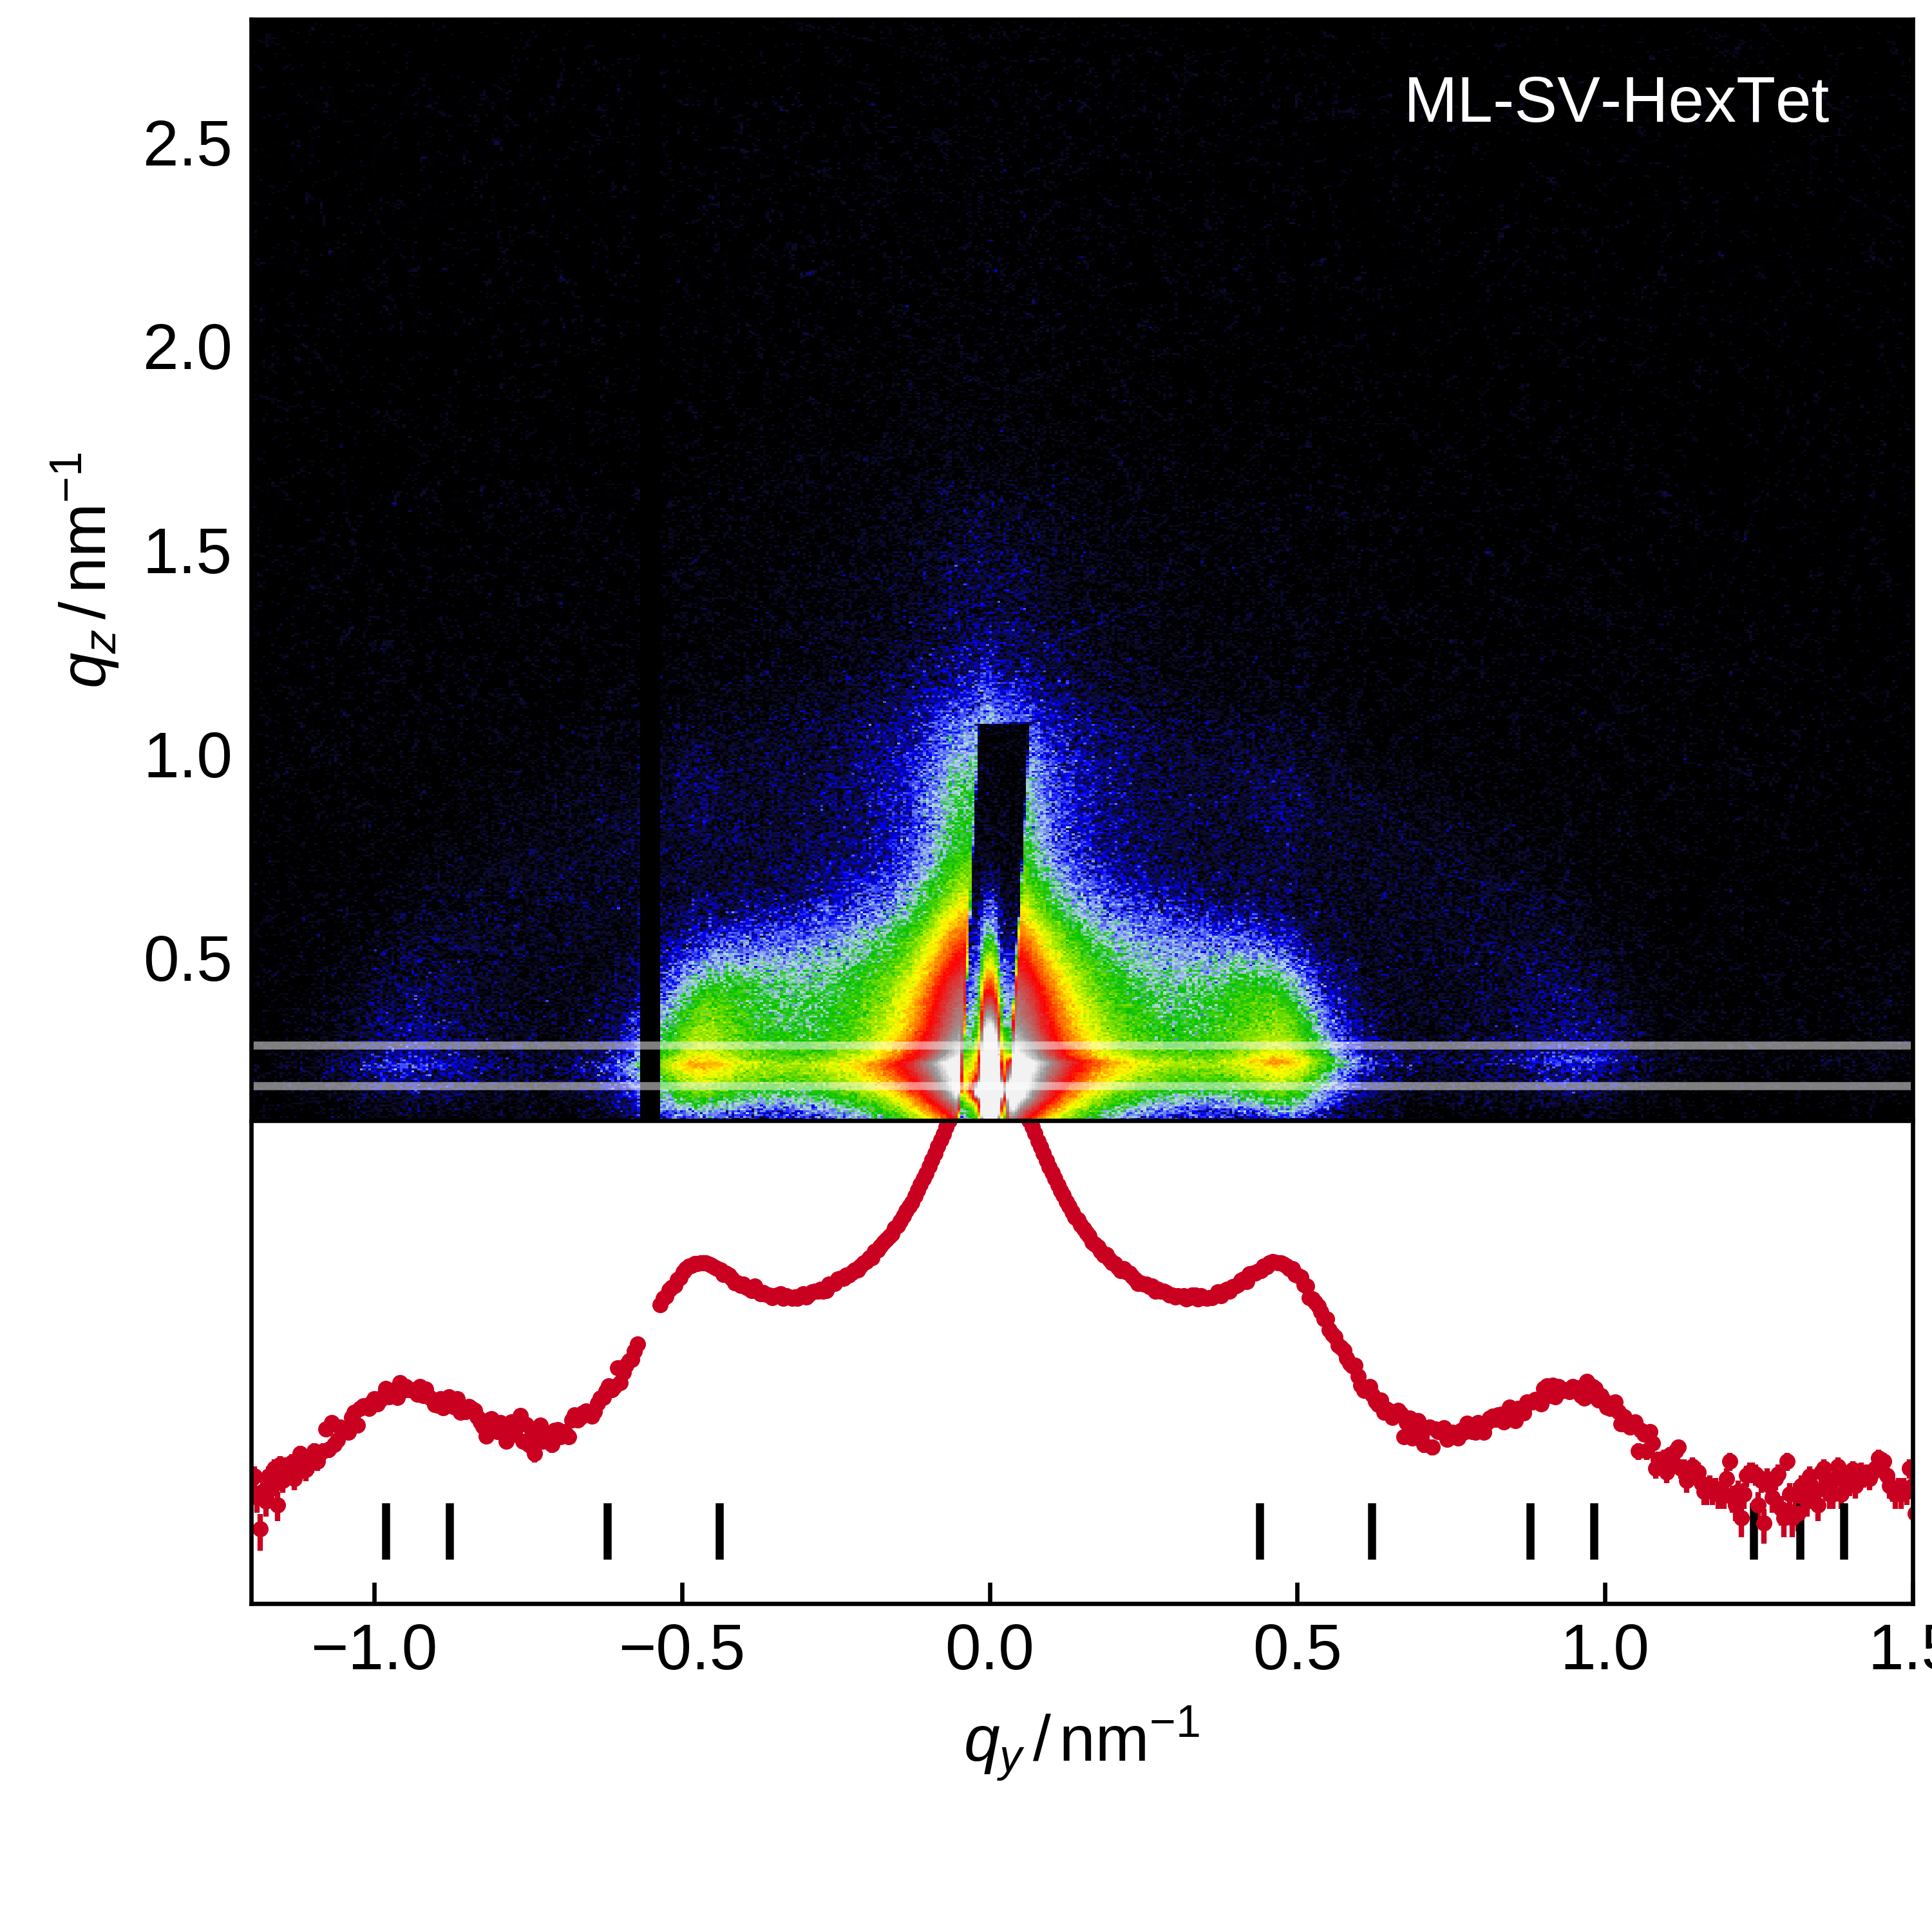
\includegraphics{monolayers_GISAXS_ML-SV-HexTet}
      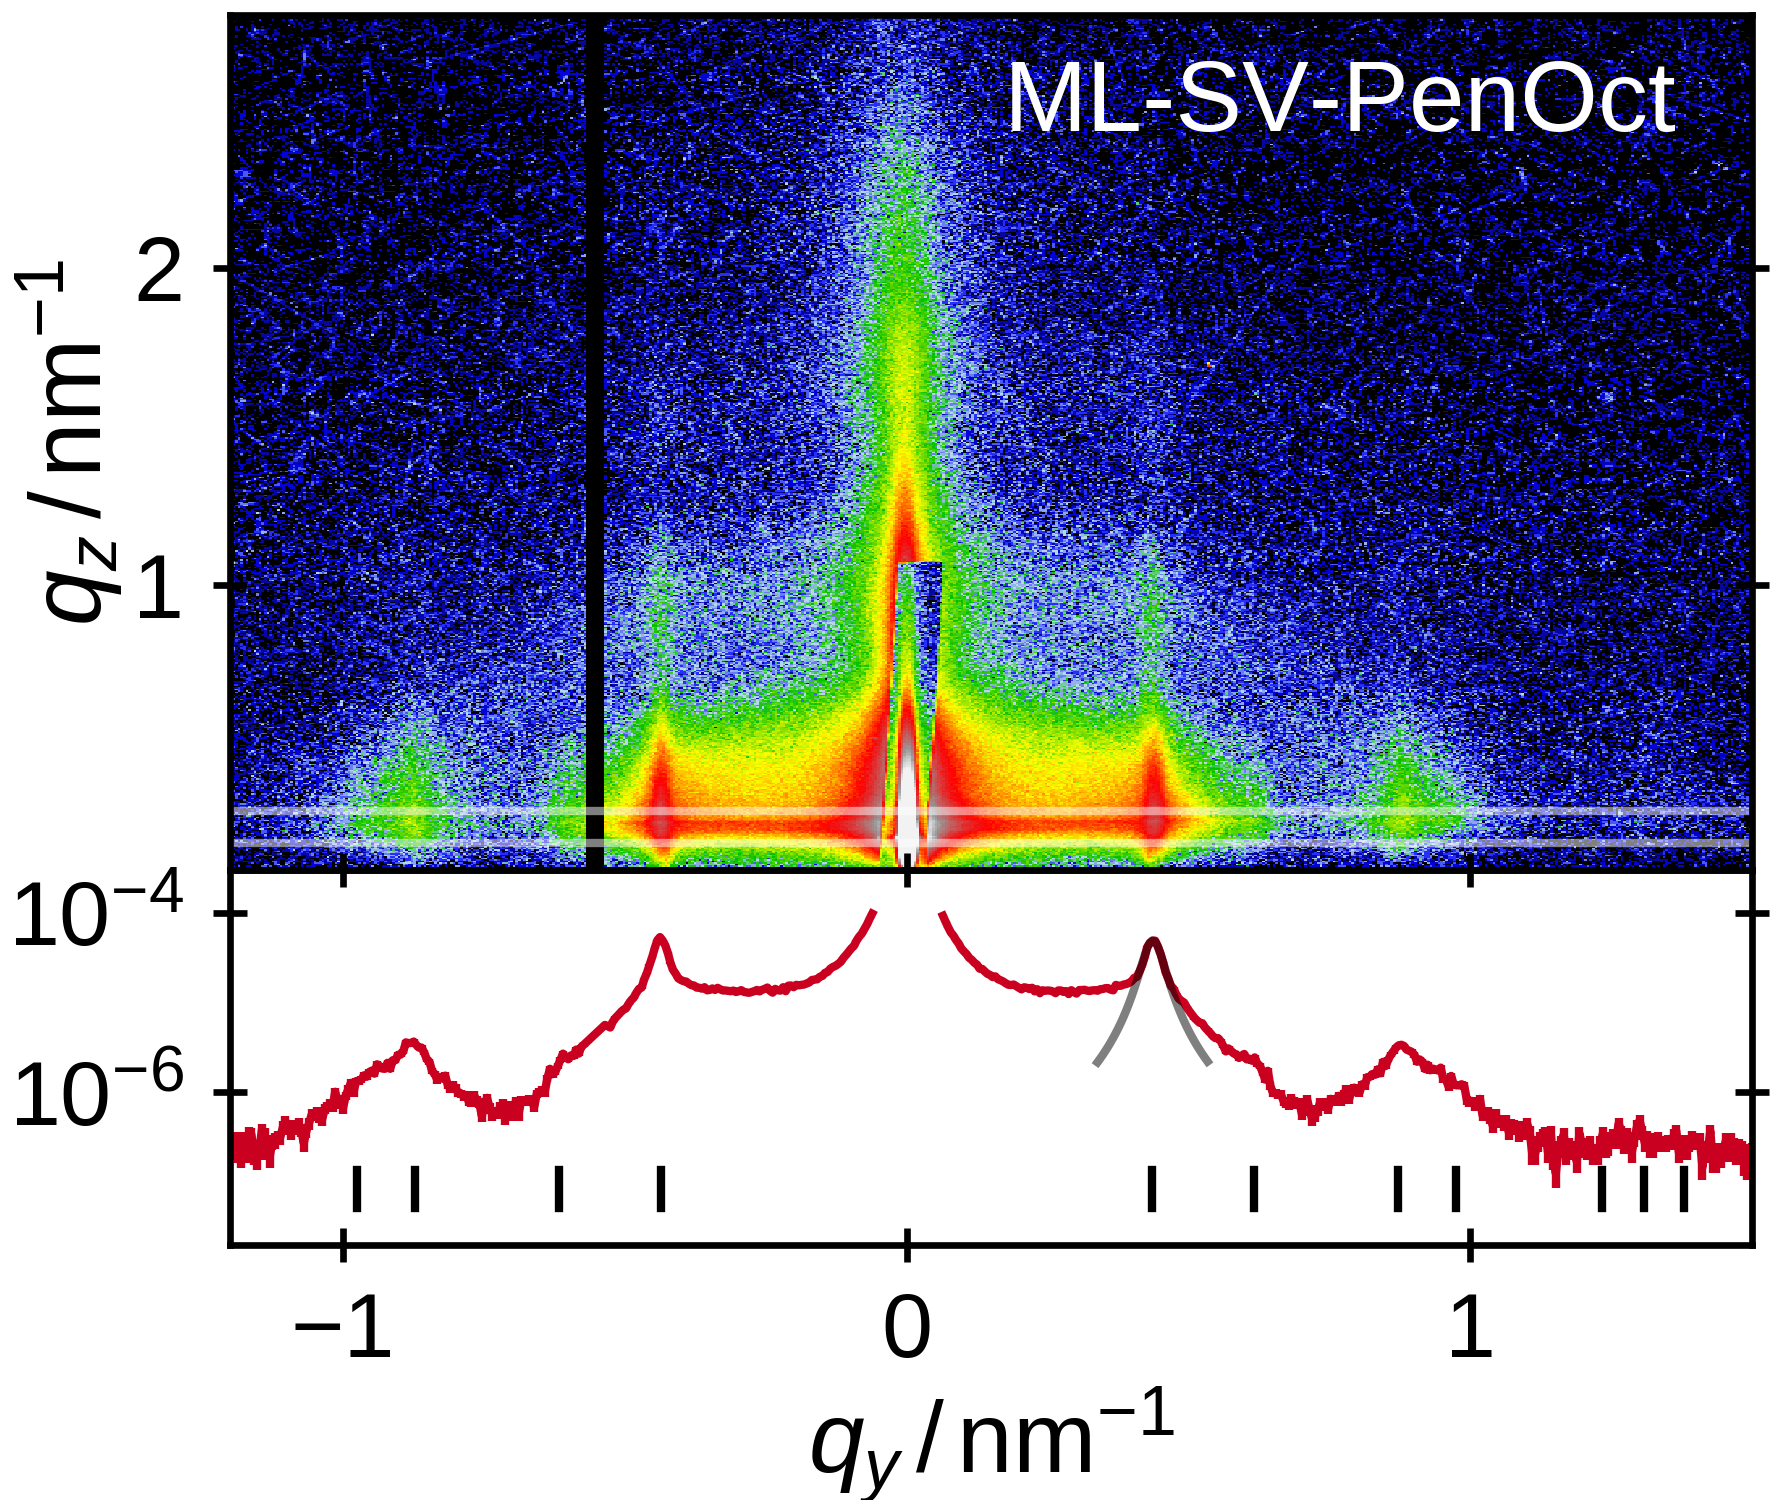
\includegraphics{monolayers_GISAXS_ML-SV-PenOct}
      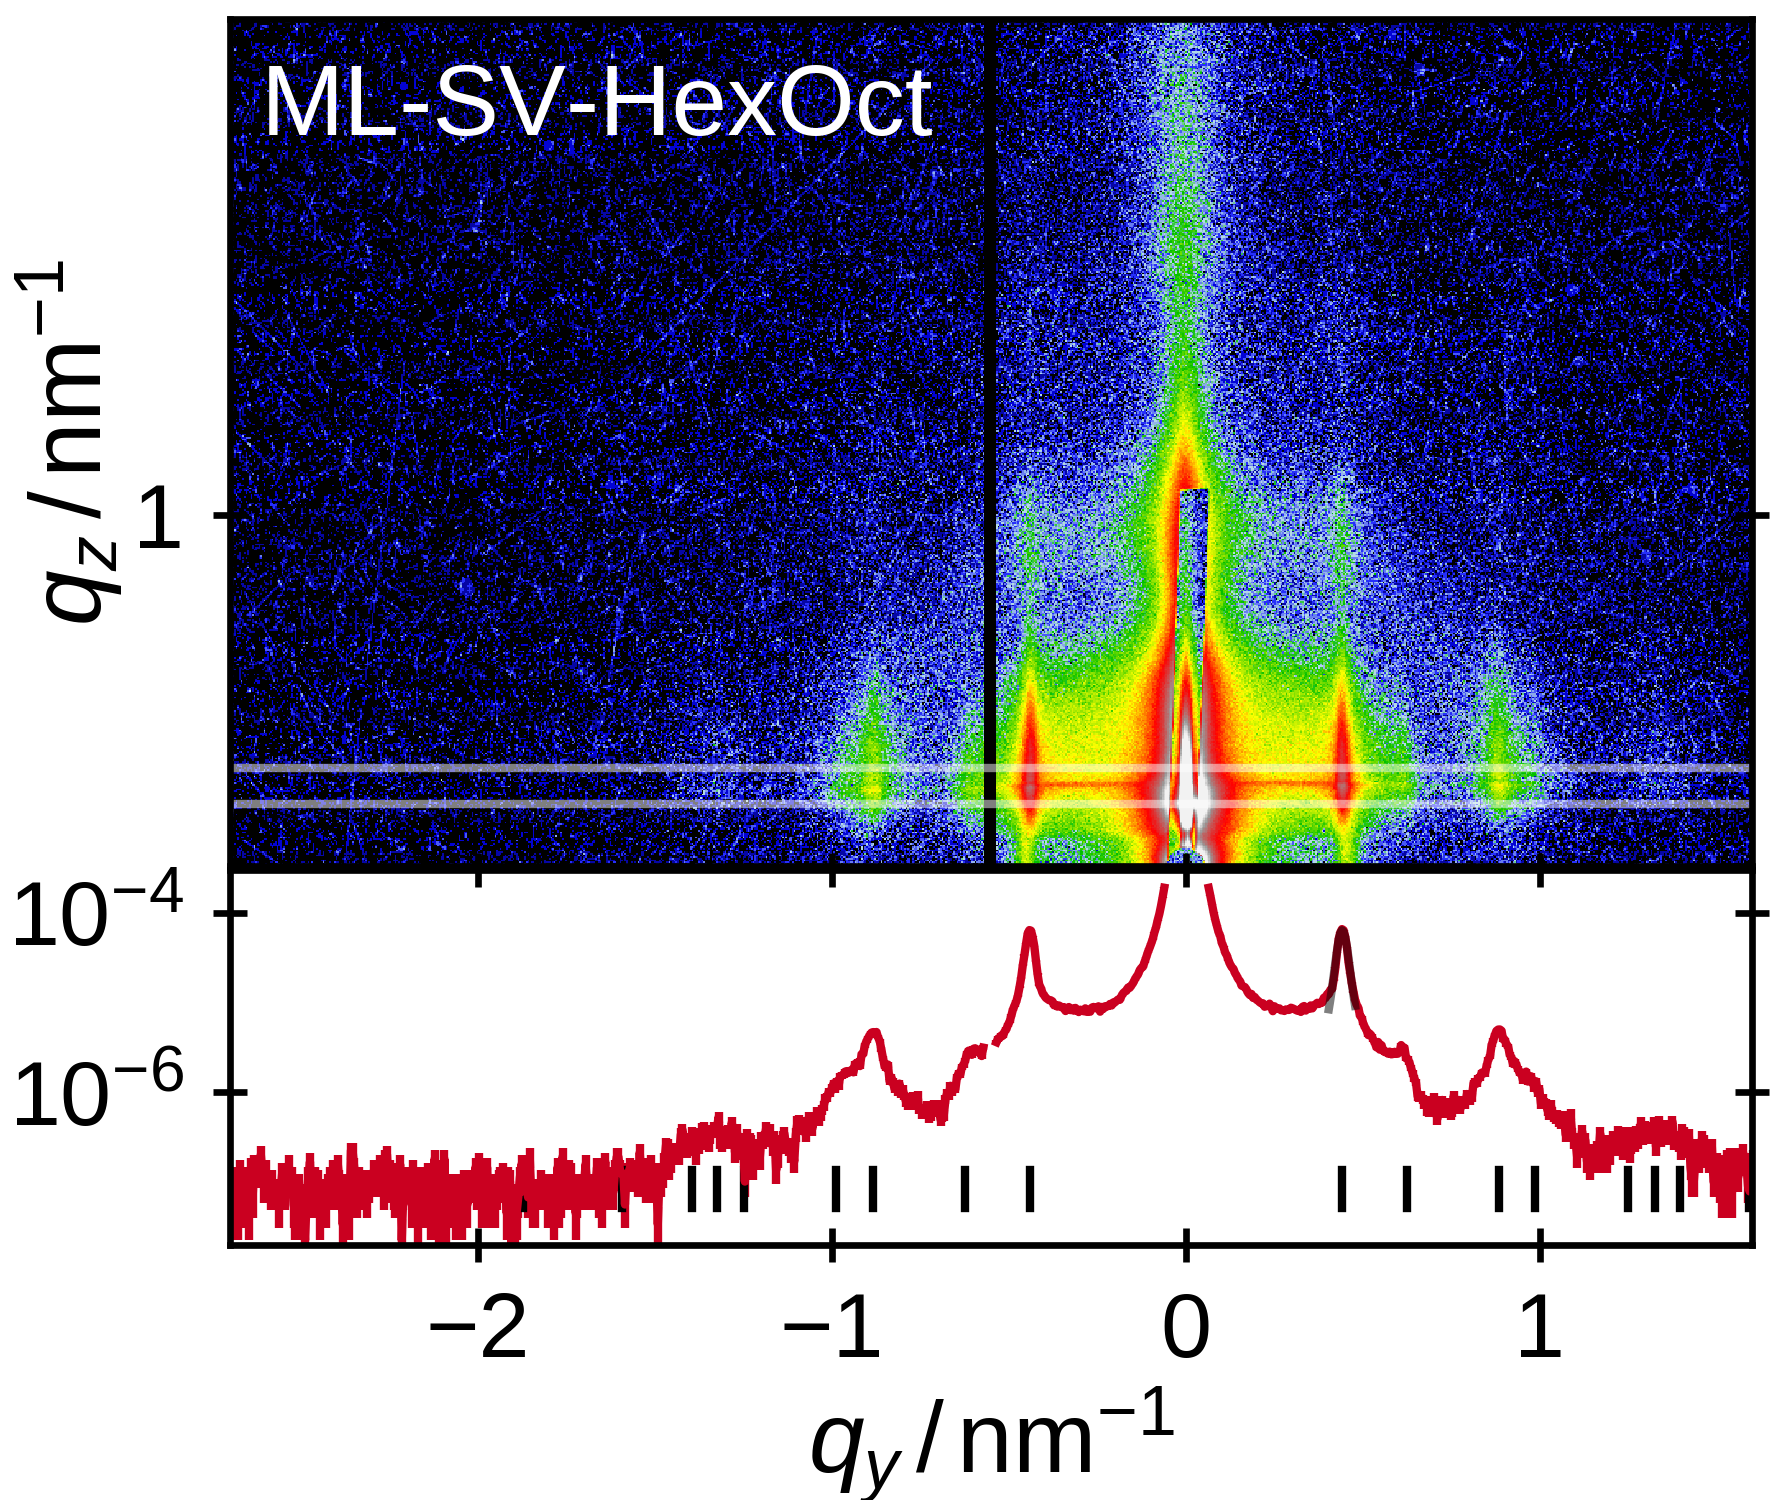
\includegraphics{monolayers_GISAXS_ML-SV-HexOct}
      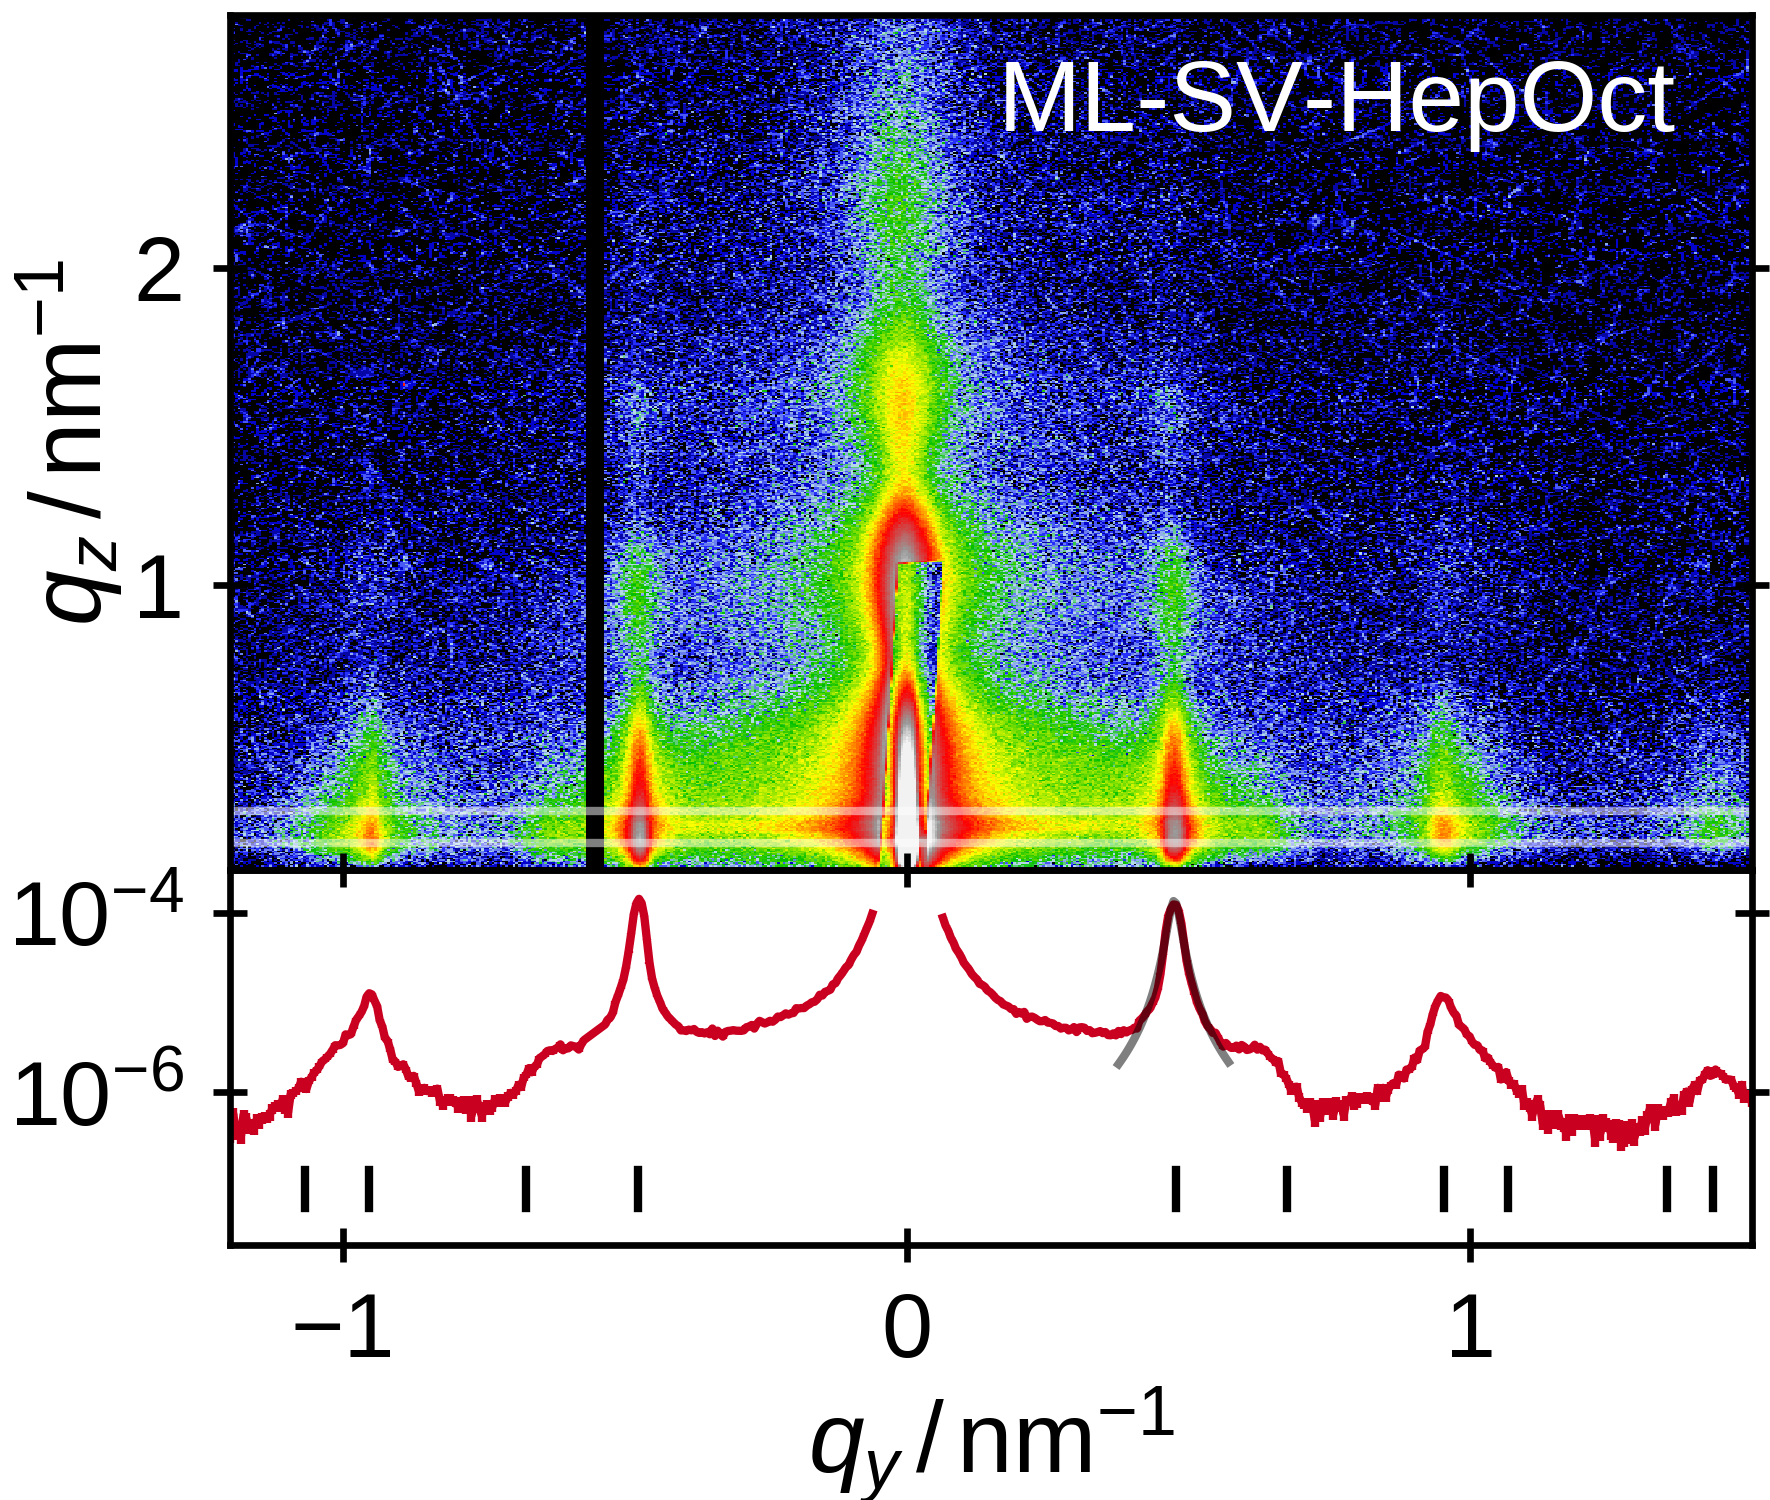
\includegraphics{monolayers_GISAXS_ML-SV-HepOct}
      \caption{\label{fig:monolayers:preparation:solventVariation:gisaxs}GISAXS detector images measured under an incident angle of $\alpha_i \eq 0.11^\circ$ to study the average lateral structure of the samples shown in \reffig{fig:monolayers:preparation:solventVariation:sem}. Below the detector images, the respective scattering intensity in the strip around the Yoneda line is shown. The first order reflection is fitted to a Voigt function with the refined parameters for the reflection position and Lorentzian broadening tabulated in \reftab{tab:monolayers:solventProperties:GisaxsLatticeParams}.}
    \end{figure}

    To quantify the in-plane order, the presented samples are studied using grazing incidence small-angle X-ray scattering at GALAXI (\refsec{ch:lss:galaxi}), shown in \reffig{fig:monolayers:preparation:solventVariation:gisaxs}.
    ML-SV-HexTet shows no significant long-range ordered structure factor in the Yoneda band, but mainly scattering coming from the form factor of the individual nanoparticles and a modulation by a short-ranged structure factor.
    For the remaining three samples distinct reflections emerge on top, which increase in intensity and sharpen for higher order alkanes.
    The first order reflection of the structured monolayers is fit by a Voigt function to determine it's center position  $q_{10}$ and it's Lorentzian broadening $\gamma_{10}$ while accounting for the finite instrumental resolution by a Gaussian broadening of $\sigma_G \eq 0.0084 \unit{nm^{-1}}$.
    The obtained (10) reflection positions, as well as the Lorentzian broadening are both tabulated in \reftab{tab:monolayers:solventProperties:GisaxsLatticeParams} for the four samples.
    The expected reflection positions for a square array are deduced from $q_{10}$ and indicated as black bars below the projected intensity of the Yoneda line.
    For ML-SV-PenOct, ML-SV-HexOct and ML-SV-HepOct the position of all reflections fit to the square array pattern.
    For ML-SV-HexTet, the (11) reflection is not observed, which further indicates that no long-range order is obtained in this sample.

    \begin{table}[tb]
      \centering
      \caption{\label{tab:monolayers:solventProperties:GisaxsLatticeParams}Scattering vector $q_{10}$ and reflection width $\gamma_{10}$ of the first order reflection observed in the GISAXS detector images in \reffig{fig:monolayers:preparation:solventVariation:gisaxs}. From the scattering vector, the lattice constant $a$ is determined and from the reflection width, the coherence length $L_{\mathrm{coh.}}$ is calculated.}
      \begin{tabular}{ c | l | l || l | l | l}
        \textbf{GISAXS}  & $q_{10} \,/ \unit{nm^{-1}}$ & $\gamma_{10} \, / \unit{nm^{-1}}$ & $a\, / \unit{nm}$ & $L_{\mathrm{coh.}}\, / \unit{nm}$ & $\sigma_\mathrm{n.N.} \, / \unit{nm}$ \\
        \hline
        ML-SV-HexTet    & $0.4617(11)$   & $0.113(4)$    & $13.61(3)$    & $348(11)$   & $2.69(4)$\\
        ML-SV-PenOct    & $0.4362(7)$    & $0.039(2)$    & $14.40(2)$    & $1010(64)$  & $1.72(5)$\\
        ML-SV-HexOct    & $0.4417(4)$    & $0.023(1)$    & $14.23(1)$    & $1710(95)$  & $1.30(4)$\\
        ML-SV-HepOct    & $0.4749(3)$    & $0.015(7)$    & $13.23(1)$    & $2623(119)$ & $0.94(2)$\\
        \hline
      \end{tabular}
    \end{table}

    A close inspection of the reflection positions and width in \reftab{tab:monolayers:solventProperties:GisaxsLatticeParams} shows that for increasing order of the alkane in the 1-octadecene samples, the lattice constant reduces and the coherence length increases.
    Both can be explained by an improved packing of the square lattice and indicates that higher alkanes increase the long-range order.
    Combining furthermore the lattice constant and coherence length to the uncertainty in the nearest neighbour position $\sigma_\mathrm{n.N.}$ using \refeq{eq:monolayers:preparation:solventVariation:RelationGammaASigma}, ML-SV-HexTet can be included in this series as the sample with the lowest degree of order.
    Finally, this quantitatively supports the qualitative observation made by SEM and reveals that the combination of \textit{n}-heptane with 1-octadecene yields the highest quality square arrays for the tested combinations.
  \FloatBarrier
\end{document}